\documentclass{beamer}
\usepackage[orientation=portrait,size=custom,width=70,height=90, scale=1.0,debug]{beamerposter}
\mode<presentation>{\usetheme{ZH}}
\usepackage{chemformula}
\usepackage[utf8]{inputenc}
\usepackage[german, english]{babel} % required for rendering German special characters
\usepackage{siunitx} %pretty measurement unit rendering
\usepackage{hyperref} %enable hyperlink for urls
\usepackage{ragged2e}
\usepackage[font=scriptsize,justification=justified]{caption}
\usepackage{array,booktabs,tabularx}

\newcolumntype{Z}{>{\centering\arraybackslash}X} % centered tabularx columns
\sisetup{per=frac,fraction=sfrac}

\newcommand{\newl}{\newline}
\newcommand{\bm}{\mathbf}
\newcommand{\bW}{\bm{W}}
\newcommand{\bV}{\bm{V}}
\newcommand{\bD}{\bm{D}}
\newcommand{\bx}{\bm{x}}
\newcommand{\bh}{\bm{h}}
\newcommand{\bz}{\bm{z}}
\newcommand{\bb}{\bm{b}}
\newcommand{\mbC}{\mathbb{C}}
\newcommand{\mbR}{\mathbb{R}}

\title{GATED COMPLEX RECURRENT NEURAL NETWORKS}
\author{Wolter Moritz, Yao Angela}
\institute[ETH]{Institute for Computer Science, Bonn University}
\date{\today}

% edit this depending on how tall your header is. We should make this scaling automatic :-/
\newlength{\columnheight}
\setlength{\columnheight}{75cm}

\begin{document}
\begin{frame}
\begin{columns}
    \begin{column}{.43\textwidth}
        \begin{beamercolorbox}[center]{postercolumn}
            \begin{minipage}{.98\textwidth}  % tweaks the width, makes a new \textwidth
                \parbox[t][\columnheight]{\textwidth}{ % must be some better way to set the the height, width and textwidth simultaneously
                    \begin{myblock}{Abstract}
                        Complex numbers have long been favored for digital signal processing, yet complex representations rarely appear in deep learning architectures.  RNNs, widely used to process time series and sequence information, could greatly benefit from complex representations.  We present a novel complex gated recurrent cell.  When used together with norm-preserving state transition matrices, our complex gated RNN exhibits excellent stability and convergence properties.  We demonstrate competitive performance of our complex gated RNN on the synthetic memory and adding task, as well as on the real-world task of human motion prediction.
                    \end{myblock}\vfill
                    \begin{myblock}{Introduction}
                        \begin{itemize}
                            \item Complex cell states can be more expressive than real ones. In GRU like RNNs the number of parameters is dominated by the weight matrices, which process the cell state. If the state size is $h_r$, these matrices have $h_r^2$ parameters. In the complex case these matrices have $2h_c^2$ parameters. For a complex network to have approximately the same amount of parameters the state can be chosen to be up to  $h_c = \sqrt{h_r^2/2}$, this is more than $h_r/2$. Counting magnitude and phase we gain some extra space.
                            \item Orthogonal and unitary matrices have been shown to be beneficial in machine learning\cite{Arjovsky,Wisdom,Hyland}. Unitary matrices are more 
                                  expressive than orthogonal ones, because their eigenvalues can be spread out over the entire unit circle, while orthogonal matrix eigenvalues are
                                  constrained to $-1, 1$.
                        \end{itemize}
                    \end{myblock}\vfill
                    \begin{myblock}{Contribution}
                            \begin{itemize}
                                \item We introduce a novel complex-gated recurrent unit to the best of our knowledge, we are the first to explore such a structure using complex number representations.  
                                \item We compare experimentally the effects of a bounded versus unbounded non-linearity in recurrent networks, finding evidence countering the commonly held heuristic that only bounded non-linearities should be applied in RNNs.  Unbounded non-linearities, in our case, perform better, but must be coupled with the stabilizing measure of using norm-preserving state transition matrices.
                                \item Our complex gated network is stable and fast to train; it outperforms state-of-the-art with equal parameters on both synthetic tasks and the real-world application of predicting poses in human motion capture.   
                            \end{itemize}
                    \end{myblock}\vfill
                    \begin{myblock}{Non-linearities}
                            \vspace{0.25em}
                            \begin{figure}
                                \begin{minipage}{0.43\textwidth}
                                    \centering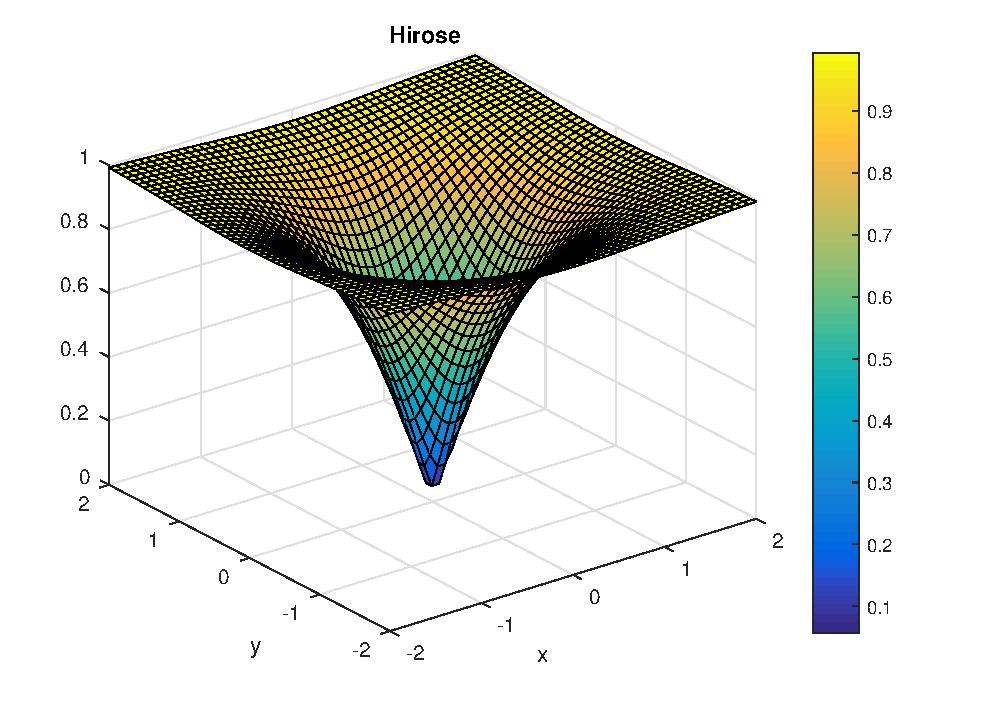
\includegraphics[width=1.0\textwidth]{img/Hirose_slice}
                                    \caption{Hirose non-linearity}
                                \end{minipage}
                                \hspace{1em}
                                \begin{minipage}{0.45\textwidth}
                                    \centering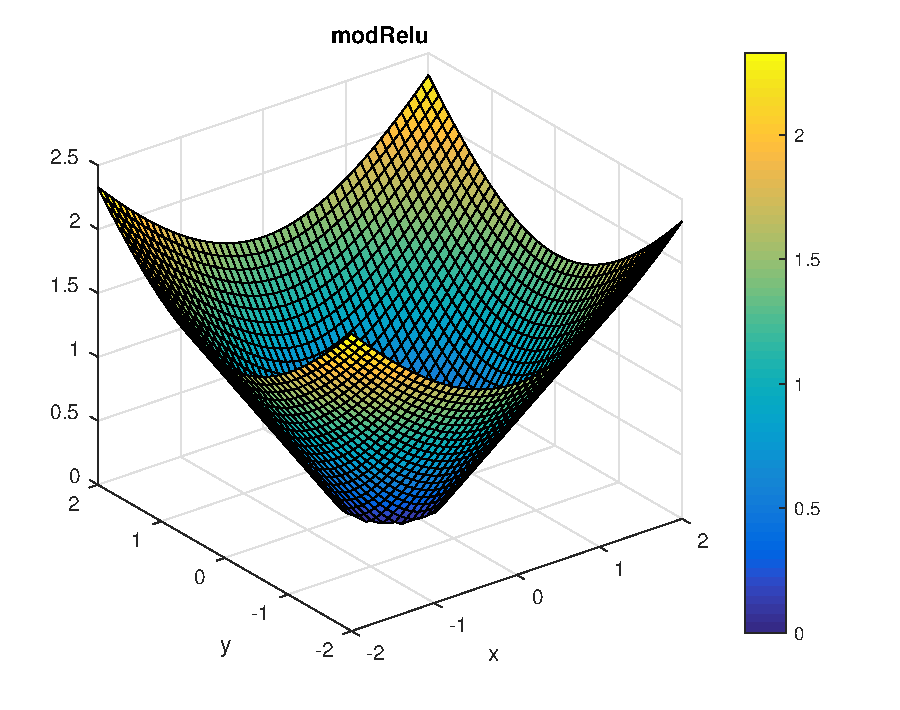
\includegraphics[width=1.0\textwidth]{img/modRelu_slice}
                                    \caption{mod-Relu non-linearity}
                                \end{minipage}
                            \end{figure}
                            \begin{equation}~\label{eq:Hirose}
                                        f_{\text{Hirose}}(z) = \tanh\left(\frac{|z|}{m^2}\right)e^{-i \cdot \theta_z} = \tanh\left(\frac{|z|}{m^2}\right)\frac{z}{|z|}.
                            \end{equation} 
                            \begin{equation}~\label{eq:modrelu}
                                        f_{\text{modReLU}}(z) = \text{ReLU}(|z| + b)e^{-i \cdot \theta_z} = \text{ReLU}(|z| + b)\frac{z}{|z|},
                            \end{equation}
                            We compare the bounded non-linearity defined in equation~\ref{eq:Hirose} as well as the unbounded one from equation~\ref{eq:modrelu}.
                    \end{myblock}\vfill
                    \begin{myblock}{References}
                        \footnotesize
                        \bibliographystyle{abbrv}
                        \bibliography{./bib}
                    \end{myblock}\vfill

            }\end{minipage}\end{beamercolorbox}
    \end{column}
    \begin{column}{.57\textwidth}
        \begin{beamercolorbox}[center]{postercolumn}
            \begin{minipage}{.98\textwidth} % tweaks the width, makes a new \textwidth
                \parbox[t][\columnheight]{\textwidth}{ % must be some better way to set the the height, width and textwidth simultaneously
                    \begin{myblock}{The complex gated RNN}
                        Following \cite{Arjovsky} we compute our weight updates using:
                        \begin{equation}
                        \mathbf{W}_{k+1} =  (\mathbf{I} + \frac{\lambda}{2}\mathbf{A}_k)^{-1}(\mathbf{I} - \frac{\lambda}{2}\mathbf{A}_k)\mathbf{W}_k \qquad \text{where} \qquad \mathbf{A} = \mathbf{W}\nabla_{\overline{\bm{w}}}{F} - \overline{\mathbf{W}}\nabla_{{\bm{w}}}{F}
                        \label{eq:Stiefel}
                        \end{equation}
                        Inspired by \cite{cho-al-emnlp14} we define our complex memory cell as: 
                        \begin{align}
                            \widetilde{\bz}_{t} &= \bW (\bm{g}_r \odot \bh_{t-1}) + \bV \bx_{t} + \bb \label{eq:state_candidate} \\
                            \bh_{t} &= \bm{g}_z \odot f_a(\widetilde{\bz}_t) +(1 - \bm{g}_z) \odot \bh_{t-1}, \label{eq:state_update}
                        \end{align}
                        With $f_a$ being the Hirose and modRelu non-linearities. We define our gates as:
                        \begin{align}
                            \bm{g}_r = f_g(\bz_r), \qquad \text{where} \qquad \bz_r = \bW_r \bh + \bV_r \bx_t + \bb_r, \label{eq:dual_gate1} \\
                            \bm{g}_z = f_g(\bz_z), \qquad \text{where} \qquad \bz_z = \bW_z \bh + \bV_z \bx_t + \bb_z.
                            \label{eq:dual_gate2}
                        \end{align}
                        Using the two gate-non-linearities:
                        \begin{align}
                            f_{g\text{ sum}}(\bz) &= \sigma(\alpha \Re(\bz) + (1 - \alpha) \Im(\bz)) \\
                            f_{g\text{ prod}}(\bz) &= \sigma(\Re(\bz)) \sigma(\Im(\bz)) \\
                        \end{align}
                        With $\alpha \in [0, 1]$. We have observed that the product formulation performs better on the adding problem, while the sum tends to do better on the memory problem. Both activations define mappings from $\mathbb{C} \rightarrow \mathbb{R}$.

                    \end{myblock}\vfill
                    \begin{myblock}{Adding and memory problem}
                        \begin{figure}
                            \begin{minipage}{0.43\textwidth}
                                \centering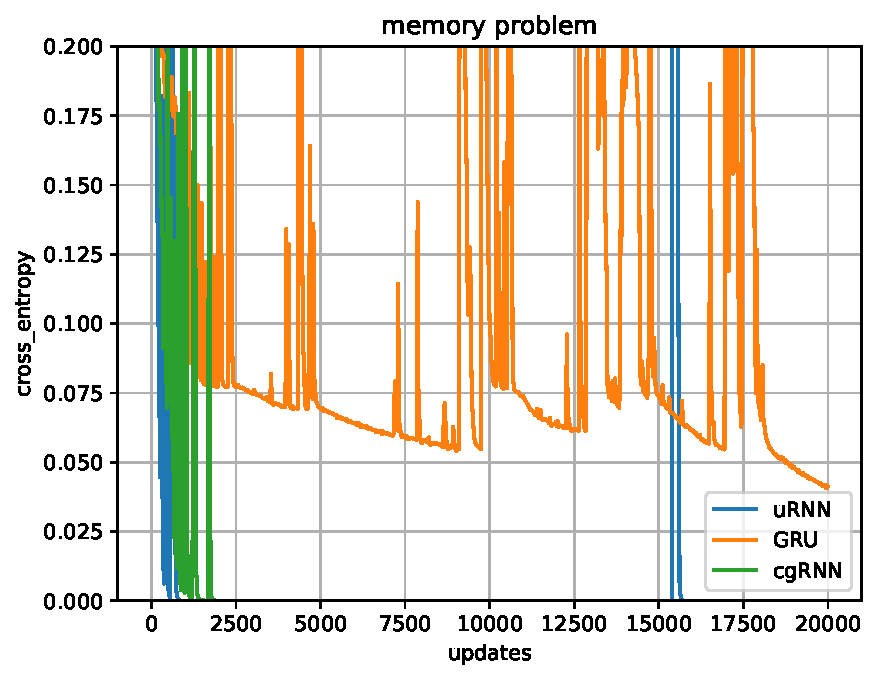
\includegraphics{img/icvss_memory.pdf}
                            \end{minipage}
                            \hspace{1em}
                            \begin{minipage}{0.45\textwidth}
                                \centering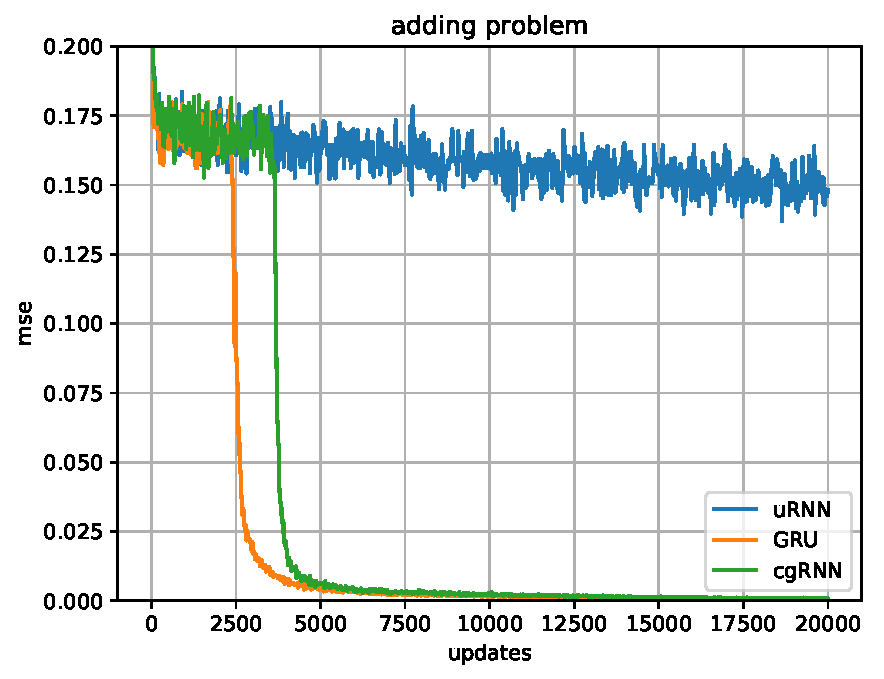
\includegraphics{img/icvss_adding.pdf}
                            \end{minipage}
                            \caption{Comparison of the previously proposed uRNN\cite{Arjovsky}(blue, $n_h=112$), %$n_h= 140$),
                             GRU\cite{cho-al-emnlp14}(orange, $n_h=112$) and our own cgRNN(green, $n_h=80$)} %all models have approximately 40k parameters.}
                        \end{figure}
                        \vspace{0.25em}
                        \begin{figure}
                            \begin{minipage}{0.43\textwidth}
                                \centering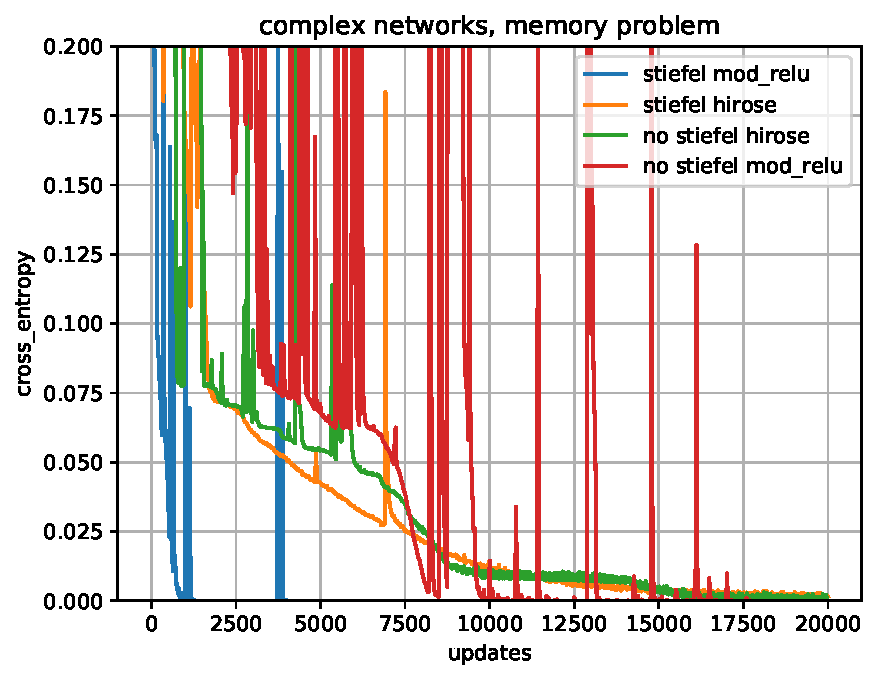
\includegraphics{img/memory_c.pdf}
                            \end{minipage}
                            \hspace{1em}
                            \begin{minipage}{0.45\textwidth}
                                \centering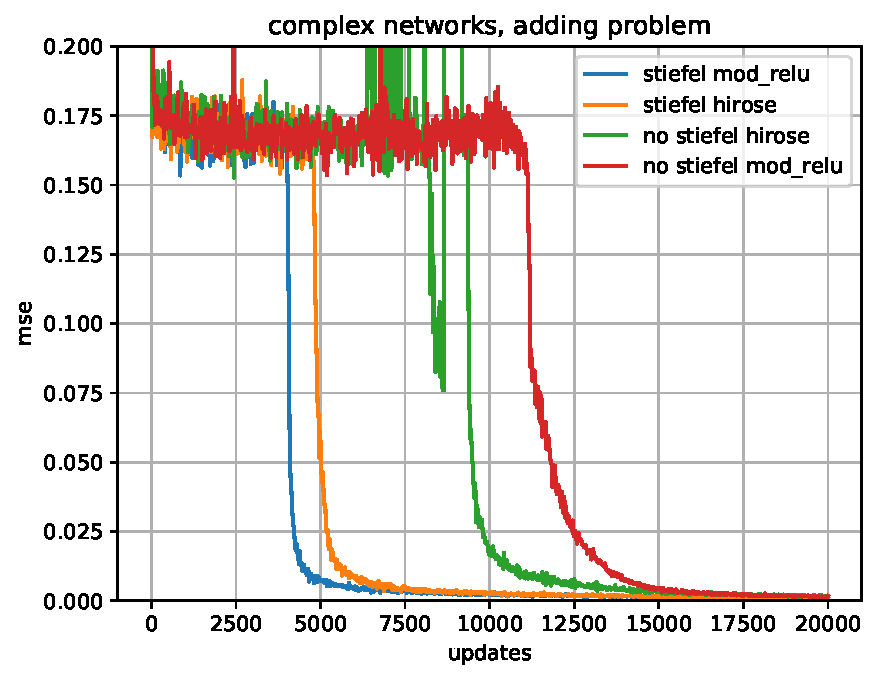
\includegraphics{img/adding_c.pdf}
                            \end{minipage}
                            \caption{Comparison of non-linearities and norm preserving state transition matrices on the complex gated RNNs for the memory (left) and adding (right) problems for T=250.  We find that the unbounded modReLU (see Eq.~\ref{eq:modrelu}) performs best for both problems, but only if the state transition matrices are kept unitary.  Without unitary state-transition matrices, the bounded Hirose non-linearity (see Eq.~\ref{eq:Hirose}) performs better. We use $n_h=250$ for the memory and $n_h=91$ for the adding problem.}
                        \end{figure}
                    \end{myblock}\vfill
                    \begin{myblock}{Human motion prediction}
                        \begin{figure}
                        \centering
                            \begin{minipage}{0.25\textwidth}
                                \scriptsize
                                \begin{tabular}{|c|c|c|}\hline
                                    seed     &   cgRNN-error                    & GRU-error                      \\ \hline
                                    0080     &   \textbf{1.13}                  & 1.24                           \\
                                    0160     &   \textbf{1.14}                  & 1.30                           \\
                                    0320     &   \textbf{1.19}                  & 1.31                           \\
                                    0400     &   \textbf{1.17}                  & 1.34                           \\
                                    0560     &   \textbf{1.23}                  & 1.39                           \\
                                    1000     &   \textbf{1.39}                  & 1.51                           \\ \hline
                                    average  &   \textbf{1.21}                  & 1.35                           \\ \hline
                                    %\bottomrule
                                \end{tabular}
                            \end{minipage}
                            \begin{minipage}[c]{.45\textwidth}
                            \centering
                            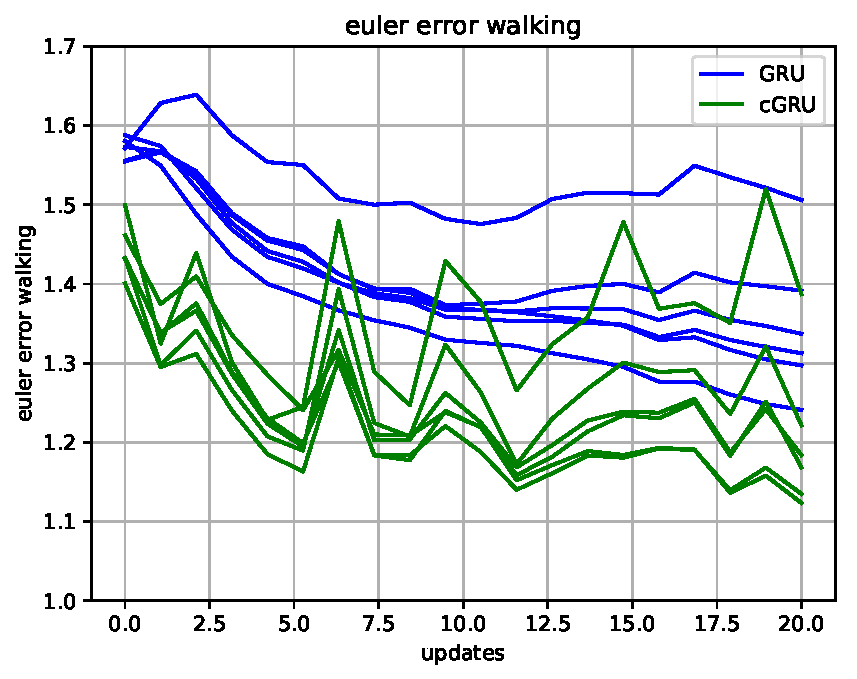
\includegraphics[scale=1.0]{img/euler.pdf}
                            \end{minipage}
                            \caption{Motion prediction Euler angle errors for the complex gated RNN (green) versus GRU (blue), where
                                     each line indicates a separate test sequence. The final error after 20000 iterations is shown in the table.}
                        \end{figure}
                    \end{myblock}\vfill
        }\end{minipage}\end{beamercolorbox}
    \end{column}
\end{columns}
\end{frame}
\end{document}